\chapter{}\label{chap1}
\addtocontents{toc}{\medskip}
\addtocontents{toc}{\protect\contentsline{chapter}{\protect \centerline{Chapter \numberline{\thechapter}}}{}}  
\addtocontents{toc}{\bigskip}

\heading{Prelude}
\smallskip

\addtocontents{toc}{\protect\contentsline{section}{\protect Prelude}{\thepage}}

\lhead[{\it\fontsize{9pt}{9pt}\selectfont\thepage}]{\it{\fontsize{9pt}{11pt}\selectfont Prelude}}

\index{Raman, Chandrasekhara Venkata!Raman Effect}

\noindent
Chandrasekhara Venkata Raman (C.V. Raman) startled the scientific world in 1928 when he announced his discovery of the  light-scattering effect named after him. The discovery was the culmination of seven years of dedicated work on the subject of light-scattering by Raman and his band of devoted students and co-workers.

Very soon after the discovery, R.W. Wood,\index{Wood, R.W.} then Professor of Physics at Johns Hopkins University\index{Johns Hopkins University} in Baltimore, \hbox{Maryland}, sent a cable to {\em Nature}\index{Nature@\textit{Nature}} which read, ``Professor Raman's brilliant and surprising discovery that transparent substances illuminated by very intense monochromatic light scatter radiations of modified wavelength and that frequency difference between the emitted radiation and the one exciting the medium is identical with the frequency of the infra-red absorption bands, opens up a wholly new field of study of molecular structure. I have verified this discovery in every particular... It appears to me that this very beautiful discovery, which resulted from Prof. Raman's long and patient study of the phenomenon of light-scattering, is one of the most convincing proofs of the quantum theory of light which we have at the present time''.

It is of particular significance that the equipment which Raman employed for the discovery were very simple and cost only Rs. 500 at the time. Very few scientists have made such a profound discovery with such simple equipment.

In 1931, C.J. Davisson,\index{Davisson, C.J.} who shared the 1937 Nobel Prize for physics with G.P. Thomson,\index{Thomson, G.P.} commenting on ``Sir \hbox{Chandrasekhara} Venkata Raman, Nobel Laureate'' in the April 1931 issue of {\em Bell Laboratories Record},\index{Bell Laboratories Record@\textit{Bell Laboratories Record}} had this to say: ``It was remarked earlier on that the Raman experiment is a rather simple one which might have been made with equipment available in any physical laboratory at any time in recent decades. It was no accident, however, that this particular discovery was made by Raman rather than someone else. Important discoveries in physics, even quite simple ones, are usually made only by investigators who have cultivated intensively the particular field concerned, and this is strikingly true in the present instance.''

In the same article, Davisson\index{Davisson, C.J.} comments: ``It speaks well for the development of science in India that Professor Raman apparently owes little or nothing of his eminence to direct contact with physicists in other countries. His formal training was received entirely in India, and, except for a single year, he has worked only in his native land. In 1924 he attended the Toronto meeting of the British Association and afterward carried on his researches for some months at the California Institute of Technology.''

Raman was a native genius who put India on the scientific map by his own efforts. For almost six decades, Raman's personality made its deep impression on the Indian scientific scene. The story of his success has few parallels, at least in the Indian context. His achievement can only be attributed to the singular nature of his personality, and the energy and vigour with which he pursued his goals. Max Born\index{Born, Max} has said of Raman, ``There is no Indian physicist of the rank of Raman. No man can compare with regard to his vigour or intensity. This European intensity which Raman exhibits to a marked degree would make an average Indian scientist suspicious of him''.


Raman showed\index{Raman, Chandrasekhara Venkata!Traits/Interests} an uncommon ability for independent thinking right from the beginning. When he took to scientific research, he was supremely confident of outstanding achievement. He used to remark that he would bring the Nobel Prize for physics east of Suez. Rabindranath Tagore\index{Tagore, Rabindranath} had won a Nobel Prize for literature in 1913, but Raman was the first Asian to win the Nobel Prize in a scientific field. Viewed from the times in which he was born and raised, it was a statement no one lesser than Raman in determination could have~\hbox{made}.

Raman was born on November 7, 1888,\index{Raman, Chandrasekhara Venkata!Birth} in South India and died on November 21, 1970.\index{Raman, Chandrasekhara Venkata!Death} He was active as a scientist almost to the very end. 1988 marked both the birth centenary of Raman as well as the diamond jubilee of the Raman Effect.

\medskip
\heading{The scientific climate in India and British rule}
\addtocontents{toc}{\protect\contentsline{section}{\protect The scientific climate in India and British rule}{\thepage}}
\smallskip

\lhead[{\it\fontsize{9pt}{9pt}\selectfont\thepage}]{\it{\fontsize{9pt}{11pt}\selectfont The scientific climate in India and British rule}}

\noindent
India is a land of ancient civilisation and, through the ages, has produced great savants, scholars and religious preceptors. Ancient \hbox{India's} contributions to medicine and mathematics have been signi\-fi\-cant and well-documented. However, modern Science, which overtook Europe during the age of Renaissance, did not come to India until much later. This was partly due to its religious attitude and partly due to its political history.

The British introduced modern education in India around the middle of the 19th century. Three universities were set up in \hbox{Calcutta}, Madras and Bombay in 1857, patterned after the London University. By the end of the 19th century there were about 200 colleges. Most Indians who received modern education in these universities and colleges sought government jobs. The best of the crop went into the Indian Civil Service and the Financial Civil Service, the two most prestigious services under British rule. Only a few took to Science, for the pursuit of Science offered very little scope for advancement to the young and the talented.

A small number of individuals who took to Science went to\break \hbox{Europe} for higher studies and research and returned to India with doctorate degrees, before pursuing scientific and teaching careers. This trickle produced some outstanding scientists and by the dawn of the 20th century, there were, at least in Bengal, one or two\break scientific societies and a few well-known Indian scientists. The names of Sir J.C. Bose,\index{Bose, J. C.} the physicist-cum-botanist, and Sir P.C\@. Ray,\index{Ray, P.C.} the chemist, were well-known. Thus, Science in India at the time was largely the effort of a few individuals; there were no great\break laboratories, except a few fledgling scientific institutions. However, the early pioneers gave a valuable start and the English professors teaching in the colleges seem to have, by and large, encouraged the brighter students. It was in this scientific milieu that Raman blossomed.

\medskip
\heading{Family and education}
\addtocontents{toc}{\protect\contentsline{section}{\protect Family and education}{\thepage}}
\smallskip

\lhead[{\it\fontsize{9pt}{9pt}\selectfont\thepage}]{\it{\fontsize{9pt}{11pt}\selectfont Family and education}}

\index{Raman, Chandrasekhara Venkata!Education|(}

\index{Raman, Chandrasekhara Venkata!Family}

\noindent
Raman was born the second child\index{Raman, Chandrasekhara Venkata!Birth} in a family of eight children, in a village near Trichinopoly in South India, where his father,\break \hbox{Chandrasekhara} Iyer,\index{Iyer, Chandrasekhara} was a teacher in a local high school.\break \hbox{Chandrasekhara} Iyer was the first person in the family to receive an `English' education, getting his B.A. degree in Trichinopoly, while working as a teacher.

The family had only modest means, but this did not stop the progressive Chandrasekhara Iyer from giving his sons an `English' education. Iyer also seems to have had artistic inclinations, for he learned the violin and apparently played it exceedingly well. This is significant because, later, Raman, during his scientific career, studied the physics of the violin. Raman's elder brother, Subrahmanya Ayyar,\index{Ayyar, Subrahmanya} was also an expert musicologist who had mastered the violin. Not much information is available on Raman's mother, Parvathi \hbox{Ammal},\index{Ammal, Parvathi} except that she was a gentle and tolerant lady, firmly rooted in the home and family life. When a correspondent asked Raman much later in life if he came from a wealthy background, Raman seems to have heartily laughed and replied, ``I was born with a copper spoon in my mouth. At my birth my father was earning the magnificent salary of ten rupees per month!''

When Raman was four years old (1892), his father accepted a post of lecturer in mathematics and physics in the coastal town of Vishakapatnam in what is now Andhra Pradesh and moved there. Raman spent the next ten years of his life in Vishakapatnam, going through primary and secondary schools and two years of college. In January 1903 he won a scholarship and joined Presidency College\index{Presidency College} in Madras for his undergraduate studies. This institution had been set up by the British Government to provide higher and quality\break education for aspiring students in South India. In those days, it was staffed mainly by English professors. The college had also acquired a great reputation at that time because of the illustrious men it had produced. It's alumni rose to high ranks in Government Service, or became judges and lawyers. It also produced outstanding scientists, of whom C.V. Raman and S. Chandrasekhar\index{Chandrasekhar, S.} became the recipients of Nobel Prizes for Physics. Unfortunately, after India's independence, Presidency College is no more the citadel of higher education in South India it once was.

Raman entered the portals of Presidency College as a young lad of 14 and when he went into his English class for the first time he apparently created a mild sensation. The English Professor turned to him and asked if he belonged to the B.A. class, to which Raman replied, ``Yes, Sir''. Referring to this incident, Raman later wrote:
\begin{quote}
{\fontsize{10pt}{12pt}\selectfont
``Some of my pleasantest recollections of the four years I spent at the Presidency College in Madras are of extraordinary kindness and consideration which I received from the European members of staff. Their attitude seems all the more surprising when I look at the undistinguished and diminutive figure of myself thirty-five years ago, as it appears in the college photographs of those days. Wearing a linen cloth in the cylindrical style of boyhood and a home-knitted cap of wool of no particular shape, I could readily have been mistaken for a high school lad who had by accident got mixed up with a college crowd. Indeed, in the first English class I attended, Professor E.H. \hbox{Elliot}\index{Elliot, E. H.} addressing me asked if I really belonged to the junior B.A. class, and I had to answer in the affirmative. He then proceeded to inquire how
old I was.''
}\relax
\end{quote}

Raman passed the B.A. degree examination in 1904, at the age of 15, winning first place and gold medals in English and
Physics.

Although Raman\index{Raman, Chandrasekhara Venkata!Traits/Interests} possessed a superior intellectual and mental capacity, his health was not equal to them. He appeared physically frail and was considered rather a weakling. When he passed his B.A.\break examination, his teachers suggested that he should go to England for higher studies. However, the Civil Surgeon of Madras, to whom he was sent for a medical check, declared that Raman was unfit to withstand the rigours of the English climate. Therefore, all ideas of sending him abroad had to be abandoned. Much later Raman appears to have said, ``I shall ever be grateful to this man''. In retrospect, what happened to Raman was a great blessing in disguise. It enabled him to chalk out his own path for a future in research. He went ahead and took his M.A. degree in 1907 at the age of 18, again topping the class with record marks.

It is said that when he was in middle school he used to read books on Science at a level far in advance of his age and
expectation, and performed experiments with improvised apparatus at home and in school. This absorption and fascination for physics were noted by his mentors in Presidency College\index{Presidency College} and his professors exempted him from attending all Science classes, as they felt that he had nothing new to learn from their lectures. Some of the certificates that his teachers gave speak for Raman's interest in English literature and for the independence and strength of character he possessed even as a young student. ``The best student I have had in thirty years''; ``Has an unusual appreciation for English literature''; ``Possesses a remarkable facility for idiomatic expression''; ``Possessing great alertness of mind and
strong intellectual grasp''.

Research\index{Raman, Chandrasekhara Venkata!Traits/Interests} in the modern sciences was quite unknown in India in those days, but young Raman, at the age of 16 and while still a student in the M.A. class, published a paper\index{Raman, Chandrasekhara Venkata!Papers/Publications/Addresses} in that prestigious journal, the {\em Philosophical Magazine}\index{Philosophical Magazine@\textit{Philosophical Magazine}} (London), in November 1906, entitled, {\em Unsymmetrical diffraction bands due to a rectangular aperture observed when light is reflected very obliquely at the face of a prism}. This was evidently a routine class experiment in optics during which Raman discovered these bands. This observation formed the first research publication of Raman and was followed by a note in the same journal on a new experimental method for measuring surface tension. These papers were communicated by the author himself and contain no acknowledgement of help received from anyone, indicating that they were based on totally independent work by Raman.

\newpage

It is important to note that Presidency College was primarily a teaching institution at that time and had no tradition at all for research. It was therefore unusual for a young student to produce research publications and have the courage to publish them promptly in the most prestigious journal at that time. It was clear even from the beginning that Raman was cut out for independent thinking. Further, his urge to put experimental observations in print as expeditiously as possible was a trait which was crucial to his career as a physicist. Indeed, this helped him to establish his priority in the biggest discovery he was to make much later in his career.
\index{Raman, Chandrasekhara Venkata!Education|)}

Even as a student he was apparently familiar with Lord\break \hbox{Ray\-leigh's}\index{Rayleigh, Lord} scientific papers and his treatise on sound as well as with the works of Helmholtz. Much later in life Raman spoke of Helmholtz thus:
\begin{quote}
{\fontsize{10pt}{12pt}\selectfont
``Speaking of the modern world the supremest (sic) figure, in my judgement, is that of Hermann von Helmholtz.\index{Helmholtz, Hermann von} In the range and the depth of his knowledge, in the clearness and the profundity of his scientific vision, he easily transcended all other names I could mention, even including Isaac Newton. Rightly he has been described as the intellectual colossus of the nineteenth century. It was my great good fortune, while still a student at college, to have possessed a copy of an English translation of his great work {\em The Sensations of Tone}. As is well known, this was one of Helmholtz's masterpieces. It treats the subject of music and musical instruments not only with profound knowledge and insight, but also with extreme clarity of language and expression. I discovered the book myself and read it with the keenest interest and attention. It can be said without exaggeration that it profoundly influenced my intellectual outlook. For the first time I understood, from its perusal, what scientific research really meant, and how it could be undertaken. I also gathered from it a variety of problems which were later to occupy my attention and keep me busy for many years.''}\relax
\end{quote}

\newpage

\heading{Entry into the Financial Civil Service}
\addtocontents{toc}{\protect\contentsline{section}{\protect Entry into the Financial Civil Service}{\thepage}}

\index{Raman, Chandrasekhara Venkata!Financial Civil Service|(}

\lhead[{\it\fontsize{9pt}{9pt}\selectfont\thepage}]{\it{\fontsize{9pt}{11pt}\selectfont Entry into the Financial Civil Service}}
\vskip .1cm

\noindent
In those days the highest-career open to bright students was entry into the Indian Civil Service. Since entry into the I.C.S. involved some degree of training in England, this was ruled out for Raman, but he was encouraged to appear for the Financial Civil Service.\break Raman appeared for the competitive examination for the F.C.S. held in February 1907. He secured the first place and was selected. His elder brother, C. Subrahmanya Ayyar,\index{Ayyar, Subrahmanya} had already entered this service.

Just before this turn of events and immediately after graduating from the M.A. class, Raman married Lokasundari,\index{Raman, Chandrasekhara Venkata!Raman, Lokasundari} daughter of\break S. Krishnaswami Iyer,\index{Iyer, Krishnaswami} who held the post of Superintendent of Sea Customs at Madras. There was a slight hitch with regard to this marriage, for Raman and Lokasundari Ammal belonged to two different subcastes. In those days, marrying out of the sub caste was tantamount to a serious transgression of the social code. The father of the girl was apparently not a willing party to the alliance, but the mother, Rukmani Ammal,\index{Ammal, Rukmani} found young Raman quite acceptable.

The story goes that on the first occasion Raman saw \hbox{Lokasundari}, she was playing on the veena the famous Thyagaraja composition, {\em Rama ni samanam evaro}, which means ``Who is equal to you, Rama?''. Lokasundari must have hit the right chords not only on the veena but in her future husband to be, for Raman firmly resolved to take her as his partner after the meeting. Referring to this incident later, Lady Raman would often say that she did not know if Raman fell for her and the music, or for the extra allowance of Rs. 150 which the Finance Department gave its married officers. The wedding took place in Madras in 1907.\index{Raman, Chandrasekhara Venkata!Marriage}

Raman, along with his wife, arrived in Calcutta later in 1907
to join the Finance Department as an Assistant Accountant
General. He was only 18$\sfrac{1}{2}$ years old. The Ramans rented a house
in Scot's Lane, off Bowbazar Street, and it looked as if the die
was cast, that Raman would have a long career in the Finance
Department of the Government of India and progress up the
ladder with the years. But Raman's real interest was rooted in
physics and an inner urge drove him to seek an opportunity to
satisfy this inner calling. He then discovered the Indian
Association for Cultivation of Science located at 210 Bowbazar
Street, only a few blocks away from where he lived.
\index{Raman, Chandrasekhara Venkata!Financial Civil Service|)}

\smallskip
\heading{The Indian Association for Cultivation of Science}
\addtocontents{toc}{\protect\contentsline{section}{\protect The Indian Association for Cultivation of Science}{\thepage}}

\index{The Indian Association for Cultivation of Science|(}

\index{Raman, Chandrasekhara Venkata!Calcutta Days|(}

\lhead[{\it\fontsize{9pt}{9pt}\selectfont\thepage}]{\it{\fontsize{9pt}{11pt}\selectfont The Indian Association for Cultivation of Science}}

\vskip .2cm

\noindent
The Indian Association for Cultivation of Science had been
in existence since 1876, founded by a leading medical practitioner
in Calcutta, one Dr. Mahendra Lal Sircar.\index{Sircar, Mahendra Lal} He had an abiding
interest in Science and foresaw the great role Science was destined
to play in India. He wanted to create an Association combining
the features of the Royal Institution of London and the British
Association and had devoted a good part of his life to collecting
funds from several princes and prominent citizens for founding
the Association of his dream, where young aspirants could devote
their lives to the pursuit of science. The Association building had
several large halls for laboratory purposes and an excellent lecture
theatre that could accommodate a large audience. During the
lifetime of ~Mahendra Lal Sircar, he organised lecture courses for
students, himself lecturing and getting others to give popular
Science lectures. However, the dream of a research institution
remained unfulfilled during Mahendra Lal Sircar's time.

In those times, scientific research in India was non-existent
and the institution decayed in 25 years, to dusty rooms and unused
laboratories. In desperation, Mahendra Lal Sircar seems to have
declared, ``I don't know how to account for the apathy of our
people towards the cultivation of Science.\index{Proceedings of the Indian Association for Cultivation of Science@\textit{Proceedings of the Indian Association for Cultivation of Science}} Younger men must
come and step into my place and make this a great institution''.
That prophetic wish was to be fulfilled by Raman.

Mahendra Lal Sircar died in 1904 rather a disappointed man.
His son, Dr. Amrit Lal Sircar,\index{Sircar, Mahendra Lal} succeeded him as the Honorary
Secretary of the Association and was guiding the affairs of the
Association at the time Raman's attention was drawn to it. Soon
after his arrival in Calcutta, Raman one day noticed the
Association's signboard while returning home from work in a
tram car. He \hbox{immediately} alighted from the car and knocked on
the doors of the Association, full of excitement and enthusiasm.
Admitted inside by a person called \hbox{Asutosh} Dey,\index{Dey, Asutosh} who was later
to become Raman's most devoted assistant, Raman met Amrit
Lal Sircar and asked him if he could conduct research at the
Association during his spare time. The story goes that Amrit Lal
Sircar embraced Raman, exclaiming that they had been waiting
for a person like him all these years, and how happy his father
would have been to witness the entry of such a person into
the Association.

\vskip .1cm

The Association premises consisted of a dusty lecture hall
and a large laboratory with dustier equipment, most of it meant
for demonstration. However, Raman set to work with enthusiasm
and very soon started producing research papers. From 1907 to
1917, except for short absences from Calcutta on transfer to
Rangoon and Nagpur, Raman spent all his leisure time, which
meant the evenings and very late into the night daily, conducting
experiments at the Association. At that time, Raman's research
was directed to the acoustics of Indian musical instruments and
he published\index{Raman, Chandrasekhara Venkata!Papers/Publications/Addresses} his findings in foreign journals as well as in the
{\em Proceedings} and bulletins of the Association.

\vskip .1cm

All the facilities of the Association were at his disposal and
he also had the devoted and loyal assistance of Asutosh Dey,\index{Dey, Asutosh}
known to everyone in the Association as Ashu Babu. Raman soon
turned the Association into a beehive of activity. His devotion
and dedication to research attracted many young students,
teachers and professors from local colleges and the universities,
who joined him to participate in the scientific excitement
he generated.

\vskip .1cm

All this meant a different story for Lokasundari Raman,\index{Raman, Chandrasekhara Venkata!Raman, Lokasundari} a
young bride thrust into the hands of a strange young man with
a consuming passion for science. Lokasundari Raman once
described the routine of Raman thus: At 5.30 a.m. Raman goes
to the Association, returns at 9.45 a.m., bathes, gulps his food
in haste, leaves for his office, invariably by taxi to be on time
for work; at 5 p.m. he goes directly to the Association on his
way back from office and comes home at 9.30 or 10 p.m, after
spending the evening at the \hbox{laboratories} of the \hbox{Association};
Sundays are spent entirely at the Association. How could a wife
tolerate such a situation!

\vskip .1cm

It is remarkable that Lokasundari Raman went along with
\hbox{Raman} in this quest for scientific knowledge. She stood by him
devotedly throughout his life and endeared herself to all who
associated themselves with her husband. She once related, with
a smile, how difficult it was to turn Raman's attention from
scientific pursuits to the obligations of matrimony. Two sons were
born to the Ramans --- \hbox{Chandrasekhar}\index{Chandrasekhar, V.} in 1921 and Radhakrishnan\index{Radhakrishnan, V.} in 1929 --- and that, Lokasundari declared, was a
miracle, for Science was his first-love.\index{Raman, Chandrasekhara Venkata!Family}
\index{The Indian Association for Cultivation of Science|)}

\medskip
\heading{Palit Professor}
\smallskip
\addtocontents{toc}{\protect\contentsline{section}{\protect Palit Professor}{\thepage}}


\lhead[{\it\fontsize{9pt}{9pt}\selectfont\thepage}]{\it{\fontsize{9pt}{11pt}\selectfont Palit Professor}}

\noindent
Raman made such a profound impression on the leading
educationists and citizens of Calcutta that Sir Asutosh Mookerjee,\index{Mookerjee, Asutosh}
the Vice-Chancellor of the Calcutta University,\index{Calcutta University} offered him the
Sir Tarakanath Palit Professorship of Physics at the University
College of Science, Calcutta. The appointment to the chair,
however, required that the candidate should have received training
abroad. Raman refused to comply with this condition. The Vice-Chancellor
eventually changed the provisions and Raman took
the chair in 1917. His resignation from the F.C.S. meant giving up
a lucrative job in exchange for one with five times less emoluments.

When announcing his plans for filling the chair, Asutosh\break
Mookerjee\index{Mookerjee, Asutosh} stated, ``For the chair of Physics created by Sir
Tarakanath Palit, we have been fortunate enough to secure the
services of Mr. Chandrasekhara Venkata Raman, who has greatly
distinguished himself and acquired a European fame by his brilliant
researches in the domain of Physical Science, assiduously carried
on under the most adverse circumstances and amidst the distraction
of pressing official duties.

``I shall fail in my duty if I were to restrain myself in my
expression of the genuine admiration I feel for the courage and
spirit of self-sacrifice with which Mr. Raman has decided to
exchange a lucrative official appointment for a University
Professorship, which, I regret to say, does not carry even liberal
emoluments. This one\break instance encourages me to entertain the
hope that there will be no lack of seekers after truth in the Temple
of Knowledge which it is our ambition to erect.''

\vskip .1cm

The encomiums paid to Raman on this occasion were well-deser\-ved. 
The remarks made by Asutosh Mookerjee,\index{Mookerjee, Asutosh} as well as
the manner in which Raman made his decision, have a deeper
significance than what is apparent, in the context of the situation
in the country at the time. Scientific research as a whole-time
career was not heard of in those days in India and most of the
top students of the time, like Raman, drifted from college into
Government Service almost as a matter of routine. However, the
fact that Raman showed scant regard for material prospects and
did not hesitate to exchange the position he was enjoying with
an academic appointment, at the first available opportunity, is
unique. This decision of his was one of considerable significance.
Very few persons would have had the courage to do so.

\vskip .1cm

The surrender of what might be called the preferments of
office in favour of the pursuit of knowledge, especially when a
person is well settled in life, as Raman was at that time, is certainly
an act of great courage. But it is interesting to note that Raman
is reported to have remarked on one occasion, in a mood of
introspection, that Sir\break Asutosh's offer of the professorship to
an unknown government\break official was an act of great courage,
whereas his own acceptance of it without demur was just a case
of following his inclinations. Events that followed have more than
justified the hopes entertained by Asutosh Mookerjee in offering
the professorship to Raman and the ambitions that impelled the
latter to accept it.

\vskip .1cm

Prof. Raman's residence at Calcutta used to be just behind
the Association. He had, therefore, provided himself a back door
entrance by which he could enter the Association at any time of
the day or night, for he never worked according to the clock.
Asutosh Dey\index{Dey, Asutosh} (Ashu Babu), the Assistant Secretary, resided on
the premises and was ever ready to assist Raman whenever he
wished to carry out his experiments at the Association's
laboratories. Raman often used to work far into the night and,
when exhausted, sleep on a table until the astonished Ashu Babu
awakened him next morning! On most mornings he would come
in informal dress to the Association and carry on experiments
until 9.30 a.m., when he would remember his lecture engagement
at the University College of Science four miles away. A quick
return home, a few strategic sweeps of his razor a quick bath,
a hurried dressing up that included arranging the inevitable
Madras turban, and he would shout at the top of his powerful
voice, ``Ashu Babu --- taxi'', evoking an equally loud response
from Ashu Babu! Snatching his breakfast on the run, he would
rush into the Association with a sheaf of his lecture notes for
the day, jump into the waiting taxi with his laboratory attendant
Shivnandan\index{Shivnandan} and, after a hectic drive, reach the Science College
just in time to start his lecture. Such was the course and tempo
of his life throughout practically his whole stay in Calcutta.

This was the time of the non-violent, non-cooperation
movement. Sometimes bands of students, who had given up their
studies at the call of Mahatma Gandhi, used to squat in front
of the Science College in Upper Circular Road, barring entry to
professors and students alike. On most of such occasions, by
cajolement, entreaty or otherwise, `Raman Saheb', as he used
to be affectionately called in those days, would break the cordon
and rush into the classroom. Calcutta was a most exciting city
in those days, but the watchword of the demonstrators used to
be `non-violence' at any cost!

The laboratories of the physics department of the College
of\break Science, particularly the many large halls reserved for the
M.Sc.\@ scholars for their practicals, had, in 1920, a rather empty
look. The equipment for many important experiments to be
performed by the students had to be improvised. The students
had ample scope for rigging up many of the gadgets needed for
the prescribed experiments. This atmosphere of improvisation
was indeed very stimulating, as it made demands for considerable
skill on the part of the scholars as well as their guides. The
experiments so set up by one batch of students were available
to the next year's batch and so on, so that in a few year's time
the laboratories were more or less filled with all the essential
experimental arrangements for the M.Sc.\@ courses in the various
branches of Physics. These were later supplemented by standard
equipment ordered from abroad.
\index{Raman, Chandrasekhara Venkata!Calcutta Days|)}

\medskip
\heading{First trip abroad and entry into light-scattering}
\addtocontents{toc}{\protect\contentsline{section}{\protect First trip abroad and entry into light-scattering}{\thepage}}
\smallskip

\index{Raman, Chandrasekhara Venkata!Visits Abroad}

\lhead[{\it\fontsize{9pt}{9pt}\selectfont\thepage}]{\it{\fontsize{9pt}{11pt}\selectfont First trip abroad and entry into light-scattering}}

\noindent
Raman's first trip abroad was to the U.K., to attend the
Congress of Universities of the British Empire held in the summer
of 1921 at\break Oxford. He represented the University of Calcutta at
the Congress. This visit gave him an excellent opportunity to meet
the leading scientists of the British Empire, who knew about  
Raman and admired his researches at Calcutta. His lecture at the
Physical Society of London on his latest researches in Optics and
Acoustics, with experimental demonstrations, drew a large
number of physicists and was immensely appreciated.

About this time, Raman was getting deeply interested\index{Raman, Chandrasekhara Venkata!Traits/Interests} in
Modern Physics. Before long, in fact, during the return voyage,
he laid the foundations for what were to be some of his most
outstanding researches for the next few decades. An intense love
of Nature, of the beauty of natural phenomena and of colour
in scenery was one of the most prominent traits of Raman. Now,
during this voyage, he became fascinated with the deep blue colour
of the sea.

The late Lord Rayleigh\index{Rayleigh, Lord} had some years earlier explained
another natural phenomenon, {\em viz}., that the blue of the sky was
due to the scattering of sun-light by the molecules constituting
the atmosphere. Such an authority like Lord Rayleigh also arrived
at the questionable conclusion that the blue of the sea was due
to the reflection of the sky blue by the ocean's surface!

Raman's marvellous intuition led him to examine the colour
of the ocean very critically during the voyage. He used the
simplest of equipment, {\em viz.,} just a nicol prism, to help him. His
wonderful imagination now led him to eliminate the sky-light
reflected by the sea surface at the Brewsterian angle by observing
the sea surface in the crossed position of the nicol prism. He was
dismayed to find the colour of the sea persisting as a much richer
blue than that of the sky!

Even on those occasions when the sea was disturbed by
waves, he found that the deep blue of the sea itself came out
unmistakably, on quenching with the crossed nicol prism the
polarised light of the sky reflected by one side of the waves. By
the time he got back to Calcutta, he was quite convinced that
the blue colour of the sea was due to the scattering of the incident
sunlight by the molecules of liquid water and that Lord Rayleigh's
earlier suggestion was not altogether correct.

\vskip .1cm

Immediately after arriving in Calcutta, Raman started critical
laboratory experiments with samples of water kept in clean
rectangular glass vessels and illuminated laterally with a strong
parallel beam of light. He observed the track of the beam in a
perpendicular direction. During the next three or four weeks he
carried out several crucial experiments with water. The disturbing
effect of dust was eliminated by using distilled water kept at rest
for many weeks, thus allowing most of the motes time to settle
down. The lateral scattering now came out as a feeble blue track
that was very highly polarised. The intensity of scattering by water,
as observed and as calculated from the Einstein-Smoluchowski
formula (originally worked out to explain the very strong critical
opalescence of liquids at their critical temperature), was shown
to be just 160 times stronger than in pure dust-free air.

\vskip .1cm

Raman wrote his classical paper on {\em The Molecular Scattering
of Light in Water and the Colour of the Sea}\index{Raman, Chandrasekhara Venkata!Papers/Publications/Addresses} within a month of
his return to India and it was published in the {\em  Proceedings of
the Royal Society of London}\index{Proceedings of the Royal Society of London@\textit{Proceedings of the Royal Society of London}} (Vol. A. 101, 1921, pp. 64-80). Only
after sending away this paper for publication did he travel down
to South India to meet his wife.

\vskip .1cm

Soon after his return from South India, Raman started
writing out his memoir entitled {\em The Molecular Diffraction of
Light}. In its chapters, besides discussing results already obtained,
he outlined plans for the many further experimental researches
to be undertaken urgently to investigate the molecular diffraction
of light by matter in the gaseous, liquid and solid states, during
its transitions from the gaseous to the liquid and from the liquid
to the solid states; in liquid mixtures, in solutions and in relation
to chemical constitution.\index{Raman, Chandrasekhara Venkata!Papers/Publications/Addresses} In this remarkable and prophetic
memoir, Raman even discussed the possible implications of the
quantum theory in one chapter. This memoir was published by
the Calcutta University Press in February 1922, indeed as
expeditiously as it was written by the author.

This is the only book Raman wrote until he published his
{\em Physiology of Vision} in the Sixties. To the question why he had
not written books, he would reply, ``When I start to write
something, I get so many new ideas it becomes impossible to
proceed further. Then I go to the laboratory to work on the new
ideas''. From 1921 onwards, the subject of light-scattering became
the main theme of the Calcutta\break group led by Raman, which
culminated in the discovery of the\break Raman Effect.

By 1924, Raman's\index{Raman, Chandrasekhara Venkata!Awards/Distinctions} outstanding researches had won for him
world-wide recognition and the Royal Society of London
conferred on him the high distinction of `Fellow of the Royal
Society: (F.R.S.)', at the young age of 36. This was universally
hailed with enthusiasm in India as recognition of native scientific
endeavour.

\bigskip
\heading{Visit to Pasadena}
\smallskip

\addtocontents{toc}{\protect\contentsline{section}{\protect Visit to Pasadena}{\thepage}}

\index{Raman, Chandrasekhara Venkata!Visits Abroad}

\lhead[{\it\fontsize{9pt}{9pt}\selectfont\thepage}]{\it{\fontsize{9pt}{11pt}\selectfont Visit to Pasadena}}

\noindent
Very soon after he became an F.R.S., Raman was invited
by the British Association for the Advancement of Science\index{British Association for the Advancement of Science} to
inaugurate the discussion on {\em The Scattering of Light} at its session
in Toronto in June 1924. After opening the discussion at Toronto,
he travelled with the Association across Canada, and then visited
Toronto again to attend the International Congress of
Mathematicians, as a representative of the Calcutta University.
He then proceeded to Philadelphia, U.S.A.,\break to attend the Centenary of the
 famous Franklin Institute.\index{Franklin Institute} Also attending this
Centenary was the leading American physicist, R.A.\break Millikan,\index{Millikan, R.A.}
who invited Raman to spend some months as Visiting Professor
at the California Institute of Technology, Pasadena. During the
fall and winter of 1924, Raman delivered a regular course of
lectures on thermodynamics to a group of American physicists
and senior scholars at the Norman Bridge Laboratory of Physics,\index{Norman Bridge Laboratory of Physics}
Pasadena.

Commenting on two special lectures delivered by Raman
before an enthusiastic audience at the California Institute of
Technology,\index{California Institute of Technology} the local newspaper, {\em Pasadena Star News,}\index{Pasadena Star News@\textit{Pasadena Star News}} referred
to them as particularly fine speeches, understandable even to
nonspecialists. It complimented Raman on his ability to expound
on a subject with clarity and eloquence combined with a rare sense
of humour.

\begin{figure}[t]
\centering
\includegraphics[scale=1.1]{eps/4.eps}

{\fontsize{10pt}{12pt}\selectfont\em R.A. Millikan and C.V. Raman, Bangalore 1940. (Photo courtesy of California Institute of Technology Archives. Pasadena, California.)}\relax
\end{figure}

The speech given at the monthly dinner of the University
Club on the evening of November 18, 1924, was reported by the
paper in its November 19, 1924 issue under the heading `Famed
Indian Scholar is Speaker'. \textit{A Game of Chance} was Raman's
subject. ``As Professor of Thermodynamics in the University of
Calcutta, India, Dr. Raman is known as one of the foremost
authorities on natural science in Asia. He is in Pasadena as a
special lecturer on physics at California Institute of Technology,''
the paper stated.


Introducing Dr. Raman, Clinton K. Judy,\index{Judy, Clinton, K.} President of the
University Club, emphasised the privilege enjoyed by the
organisation in listening to a scientific scholar from the Orient.
``Most Hindus coming to this country talk on philosophy and
the occult, and it is a distinct novelty to have one who is more
in accord with Western scholarship,'' said Professor Judy.

Dr. Raman proved himself an entertaining speaker,
displaying a delightful strain of humour. He began by stating
that games of chance had always held a deep fascination for the
human mind. In support of this, he recalled several legends from
the ancient Sanskrit, according to which humans played at dice
with the Gods.

\vskip .06cm

Drawing interesting analogies between games of chance and
the issues of life, Dr. Raman said there really was no such thing
as chance, because everything happened for definite reasons. But
those for which the causes were not known were characterised
as chance.

\vskip .06cm

In the course of his remarks, Dr. Raman described some of
the experiments that famous mathematicians had conducted to
work out the details of the law of probabilities, recalling battles
that many University Club members themselves had fought with
sequences, choice and chance in their college days. Fascinating,
too, were his remarks on the law of irreversibility, something
which, he said, few people ever thought about.

\vskip .06cm

It was an evening of mental gymnastics, which Dr. Raman
concluded by saying, ``The greatest game of chance of all is
Nature'' --- thus adding a touch of the mystical and giving the
audience something more to think about.

\vskip .06cm

The {\em Pasadena Star News}\index{Pasadena Star News@\textit{Pasadena Star News}} dated December 19, 1924, reported
another lecture by Raman\index{Raman, Chandrasekhara Venkata!Papers/Publications/Addresses} under the headings: ``Fine Lecture
Offered By Indian, Prof. C.V. Raman of India Speaks on Light
Theories, Demonstrates Talk With Many Experiments of Keen
Interest''. It then went on to say:
\begin{quote}
{\fontsize{10pt}{11.5pt}\selectfont
``Prof. C.V. Raman, noted Indian scientist, and professor
of physics at the University of Calcutta, India, yesterday addressed
an enthusiastic audience of more than 300 teachers, students and
graduates of the California Institute of Technology on the subject
of {\em The Scattering of Light and Its Relation to Atomic and
Molecular Structure.}

The noted scientist, who has come to the Southland from
Toronto, Canada, where he recently arrived from India, received
a splendid tribute from his interested audience at the close of
his address.

Both the physicist and the chemist, Dr. Raman believes, have
left a neutral space between their theories as to the construction
of the atom, especially as those theories apply to light, and his
mission was to give each food for thought, so that the two great
sciences might be brought closer together.

Dr. Raman first developed the theory of the `scattering' of
light on a trip in the Mediterranean Sea. The deep blue of that
great body of water was a puzzle to him, and he finally solved
the mystery, at least to his own satisfaction, by proving with
hundreds of experiments, that the scattering of sunlight itself
was responsible.

His lecture was illustrated with many experiments, given in
such a simple and direct manner that they could be easily
understood by a less scientific audience than that present.

One piece of apparatus which he has invented for the study
of light-scattering in gases and vapour, is a huge black box, seven
feet in height, in which an observer may station himself, and in
which an apparatus contains the gas, air, or vapour, to be studied.
Dr. Raman, with rare humor has named this `The Black Hole
of Calcutta'.

In one demonstration, the scientist gave a remarkable view
of the setting sun, which he obtained by using a liquid encased
in a square glass receptacle in the receptor of a projector, instead
of a slide.

Dr. Raman is a graduate of the University of Madras in
Southern India, and is among the most noted teachers in the world
of science. This is his first visit to the United States and to
California and he was enthusiastic about the Southland. Interest
in his subject here surprised him; attendance at scientific lectures
in India he said being one of the much desired conditions that
is sadly lacking.''
}\relax
\end{quote}

Raman's\index{Raman, Chandrasekhara Venkata!Papers/Publications/Addresses} visit to Pasadena enabled him to develop a lifelong 
friendship with Millikan and other leading American
physicists. The admiration of Millikan for Raman is reflected
in the announcement of a lecture at California Institute of
Technology.\index{California Institute of Technology} This announcement, dated December 9, 1924, was
evidently prepared by Millikan himself.
\begin{quote}
{\fontsize{10pt}{12pt}\selectfont
``The Friday Evening Demonstration Lecture this week at
the California Institute of Technology will be one of unusual
interest, both because of the personality of the speaker, and
because of his subject. Dr. C.V. Raman, Professor of Physics at
the University of Calcutta, India, will be the speaker and his
subject is {\em The Study of Musical\break Instruments}.

Dr. Raman stands out as one of the most productive scientists
of the Orient. He has already done a surprising amount of high
grade\break scientific work himself and has stimulated a great deal more
among students. His publications on the mechanical theory of
stringed instruments have made him an internationally known
authority, upon the subject about which he is speaking. This in
itself is enough to make the lecture one of great interest, but
Dr. Raman has in addition so much personal enthusiasm for his
subject, so fine a command of the English language, and so great
an ability to present a subject in an entertaining and clear manner
that he is an exceptionally interesting speaker. He has been
lecturing this fall at the Institute upon the subject of
`Thermodynamics,' but has consented to speak at this time upon
his work on stringed instruments because of its greater popular
interest. He will illustrate his lecture with a number of unusual
experiments on stringed instruments of various sorts.

The lecture will be given in the lecture hall of the Norman
Bridge Laboratory of Physics\index{Norman Bridge Laboratory of Physics} from seven to eight o'clock, Friday
evening, December 12th. It is open to the public without charge.''
}\relax
\end{quote}

Raman returned to Calcutta in February 1925 after visiting
{\em en route} several countries of Western Europe to meet some of
the great leaders in physics, such as Niels Bohr,\index{Bohr, Niels} Max Planck,\index{Planck, Max}
Fabry,\index{Fabry, C.} Siegbahn\index{Siegbahn} and others.

Raman's first two visits abroad and the contacts he made
with many scientific men and institutions during these visits
brought about a very wholesome change in his habits and methods
of work. Previously, he used to work for very long spells, without
regard to day or night, oblivious to his needs of food, rest etc.
After his foreign experiences, the pattern of his working became
more regular and systematic. He developed more business-like
habits in getting through his very heavy work-load of scientific
research as well as direction of his many pupils. Regular hours
for meals and short spells of relaxation in the evenings must have
been a great relief to Lady Raman.

\vskip .1cm

After Raman became an F.R.S., the authorities of the
Calcutta University were pleased to augment his salary. According
to L.A. Ramdas,\index{Ramdas, L.A.} he acquired a horse and carriage about 1924,
thus freeing himself from dependence on taxis. The carriage was
black, the horse was chestnut brown and there was a syce to take
care of both and also act as driver. It was a very presentable set-up.
 Often, while taking his evening drive, and if Lady Raman
was not accompanying him, he would invite one of his senior
scholars to keep him company.

\vskip .1cm

Ramdas describes the experience of an outing with Raman
so:  ``The evening drive usually led to the Calcutta Maidan,
stopping somewhere near the statue of Lord Kitchner or Lord
Roberts. Getting down, Prof. Raman would take a brisk walk
towards Fort William and then take some quick jerks of `Kasrat'
and `Dand' for exercise. He would then walk back to his carriage
and drive home. On the occasion when I was with him, while
walking back to the carriage at a distance of half-a-mile, he
suddenly asked for the exact time. I said 7.20 p.m. He asked me
if I had a watch. I said `No' but pointed at the distant tower clock of Whiteaway and Laidlaw. He said that it takes him
exactly 12 minutes to cover the distance and would check if I was
right. To my great relief the time was 7.32 when we reached the
carriage! He complimented me on what he called my excellent
eye-sight. On the return drive we had a very interesting discussion
on our current researches at the Association, during which many
fresh lines of investigation cropped up. I did not know how the
time passed. We arrived at the Association by 8 p.m. My home
being close to Prof. Raman's, we both went home by the famous
back-gate for which I was one of the privileged few to possess
the freedom of the key.''

\medskip
\heading{Discovery of the Raman Effect}
\addtocontents{toc}{\protect\contentsline{section}{\protect Discovery of the Raman Effect}{\thepage}}
\medskip

\index{Raman, Chandrasekhara Venkata!Raman Effect|(}

\lhead[{\it\fontsize{9pt}{9pt}\selectfont\thepage}]{\it{\fontsize{9pt}{11pt}\selectfont Discovery of the Raman Effect}}

\noindent
In 1923, a detailed study of the scattering of light in water
was taken up by K.R. Ramanathan, one of the research scholars
who worked under Raman. Sunlight was focussed on the liquid
contained in a flask, and the scattered light was observed as a
track in the transverse direction. By the use of complementary
filters, in the incident and scattered direction, a residual intensity
was observed, which \hbox{Ramanathan} described as a ``weak
fluorescence'' due to the presence of impurities in the fluid.
However, even after repeated distillation of the liquids, the ``weak
fluorescence'' persisted undiminished. Raman was not satisfied
with the explanation and felt it might be something analogous
to the Compton effect\index{Compton Effect} in X-ray scattering which had just then
been discovered.

Two years later, K.S. Krishnan,\index{Krishnan, K.S.|(} another research scholar
under Raman, observed the same phenomenon while studying
the scattering of light in 65 different carefully purified liquids.
He also made another important observation, that the new
radiation was partially polarised, unlike ordinary fluorescence,
which is unpolarised. The technique used for observing the new
phenomenon made use of a beam of sunlight, a condensing lens
of large aperture, a flask containing the liquid and a set of
complementary filters, {\em i.e.} a violet-blue filter in the path of the
incident beam and a greenish-yellow filter in the path of the
transversely scattered light.

S. Venkateswaran,\index{Venkateswaran, S.} a part-time research worker at the
Association, continued the work of K.S. Krishnan in the summer
of 1925. He attempted to photograph the spectrum of the
scattered light using sunlight passed through coloured filters, but
was unable to report any decisive results. Raman, under whose
guidance all this work was conducted, was not at all satisfied with
the explanation that the feeble residual scattering was due to
fluorescence appearing in the spectrum in a region different
from that of the incident beam. He suspected it was an entirely
new type of secondary radiation, quite distinct from the usual
fluorescence which was normally of high intensity and
unpolarised.

The award of the Nobel Prize to Compton in 1927 acted as
a great impetus to Raman to seek an analogous effect with light.
One of Raman's pupils during the Calcutta days,
B.N. Sreenivasiah,\index{Sreenivasiah, B.N.} gives this eye witness account of what he saw
and heard at the Association one day towards the end of 1927:
\begin{quote}
{\fontsize{10pt}{12pt}\selectfont
``On a November evening in 1927, while I was at Calcutta
after an examination and interview at Delhi, I visited the
Association at Calcutta to pay my respects to Prof. Raman.
His elder brother, Shri C.\@ Subrahmanya Ayyar\index{Ayyar, Subrahmanya} (father of the
famous Astrophysicist, Prof.\@ S.\@ Chandrasekhar),\index{Chandrasekhar, S.} was also with
Prof.\@ Raman when I entered his office. Soon after I went
in, Dr. K.S. Krishnan rushed in and excitedly informed Professor
of the announcement in the evening papers that
Prof. A.H. Compton\index{Compton, A.H.} had been awarded the Nobel Prize in
Physics for his discovery of the Compton Effect in X-Rays. On
hearing this news, Prof. Raman beamed with delight and burst
out in his characteristic fashion: `Excellent news.... very nice
indeed. But look here, Krishnan. If this is true of X-Rays, it must
be true of light too. I have always thought so. There must be an
optical analogue to the Compton Effect. We must pursue it and
we are on the right lines. It {\em must} and shall be found. The Nobel
Prize must be won'.''}\relax
\end{quote}

And Sreenivasiah goes on to record how only a few months
later he attended an address Prof. Raman delivered in Bangalore
on {\em The New Radiation!}\index{Raman, Chandrasekhara Venkata!Papers/Publications/Addresses}

\vskip .06cm

For some years these studies seem to have been kept in the
background, while Krishnan engaged himself in some theoretical
problems. In the winter of 1927, Raman went on a vacation to
Waltair, the university town on the coast of what is now in Andhra
Pradesh. He had the Compton Effect on his mind and started
working on it in Waltair. He derived a formula for the Compton
scattering using the classical theory and this helped him to realise
that the ``weak\break fluorescence'' might be the incoherent scattering
with a change of wavelength, analogous to the Compton scattered
radiation. Back from vacation and with new insights, Raman
decided to find a satisfactory solution to the problem and asked
Krishnan to stop his work on theoretical problems and start more
intensive experimental studies on the anomalous scattering in
liquids and vapours. He put Venkateswaran\index{Venkateswaran, S.} and Krishnan on
purifying the liquids and got them to repeat the observations.
In January 1928 the former found that in pure glycerine the
scattered light was greenish in colour instead of the usual blue,
and that the radiation was strongly polarised. This gave them
a fresh impetus to attack the problem.


Raman and Krishnan set up a better scattering set-up to
examine the scattered intensity. They used a powerful beam of
sunlight,\break focussed by an 18 cm telescope objective lens combined
with a short focus lens. This was passed through a blue-violet
filter and then through the liquid (contained in a sealed flask)
purified by repeated double distillation {\em in vacuo}. When a second
filter of green glass, which was complementary in colour to the
blue-violet filter, was placed in the path of the incident beam,
no track of the scattered light was visible in the transverse
direction. When the same was placed between the bulb and the
observer, the track within the liquid continued to be visible,
though less brightly.



Krishnan confirmed on February 7, 1928 the presence of
``weak fluorescence'' observed by Ramanathan earlier in a
number of organic liquids and vapours. Nearly 80 different
aromatic, aliphatic and inorganic liquids were examined and the
effect was seen in all cases, indicating thereby the universal
character of the phenomenon. It was shown to be distinctly
different from the usual fluorescence, because of its feebleness
and strong polarisation which was nearly the same as that of the
unmodified scattered light.

Raman personally verified all these observations and
was very excited. Krishnan noted in his diary, that on the night
of February 7th, Professor Raman rushed to Krishnan's residence
to tell him that the observations they had made that morning were
related to the Kramers-Heisenberg process for which they had
been looking all these years. They christened the effect `modified
scattering'.

Two days later, Raman and Krishnan detected the new
radiation in vapours of ether and amylene. They soon realized
that they were dealing with a new phenomenon of a fundamental
character and communicated their conclusions by cable to {\em Nature}\index{Nature@\textit{Nature}}
on February 16, 1928. In a letter entitled `A New Type of
Secondary Radiation', which was published on March 31, 1928,
they repeated the arguments used in Raman's classical derivation
of the Compton effect\index{Compton Effect} and suggested that the modified radiation
could arise from the fluctuations of the molecules from the normal
state. Raman and\break Krishnan succeeded in detecting the new
radiation and in observing its partial polarisation in a number
of organic vapours as well as in the gases CO$_2$ and N$_2$O.
The modified scattering was easily detected in vapours such as
ether and pentane at higher temperatures and consequent higher
vapour pressures. Its polarisation was quite strong and was
comparable with the polarisation of ordinary scattering.

While continuing further studies on the subject, Raman and\break
Krishnan, on the afternoon of February 28, 1928, examined the
influence of the wavelength of the incident-light on the
phenomenon. Using incident radiation of a narrower range of
wavelengths brought about by a combination of blue-violet filter
and a piece of uranium glass, they examined the scattered track
through a direct vision spectroscope. To their great surprise they
found that the modified scattering was separated from the
scattering corresponding to the incident-light by a dark space.
Still, the experiments were performed with sunlight.

Further work carried out on that day was described by
Raman himself in an address given on March 16th that same year
in Bangalore. ``This encouraged me'', he said, ``to take up
observations with a monochromatic source of light. A quartz
mercury lamp, with a filter which completely cuts out all the
visible lines of wavelength longer than the indigo line 4358 A.U.,
was found to be very effective. When the light from such a lamp
was passed through the bulb containing a dust-free liquid, and
the spectrum of the scattered light was observed through a direct
vision spectroscope, it was found to exhibit two or more sharp
bright lines in the blue and green regions of the spectrum. These
lines were not present in the spectrum of the incident light or
in the unfiltered light of the mercury arc and are thus manufactured by the molecules of the liquid.''

Krishnan and Venkateswaran\index{Venkateswaran, S.} were working with Raman at
the time of the discovery and thus had the distinction of knowing
about the discovery first. Most of the other scholars in the
laboratory subsequently had the opportunity of seeing this
phenomenon on that day. By this observation, the discovery of
the new effect was complete. Raman's student Ramdas\index{Ramdas, L.A.} first called
the phenomenon the ``Raman Effect'' in his paper, {\em The Raman
Effect and the Spectrum of the Zodiacal Light}, published in
{\em Nature}, Vol. 122, p. 57, July 1928.

Prof. Raman once told me that he first saw the effect in
benzene through the direct vision spectroscope. He demonstrated
this to me one day at the Raman Research Institute.\index{Raman Research Institute} He also said
that the viewer should be in the dark room for a while and rest
the eyes to see the effect. And surely it was there in benzene. I
could see the Raman line in diamond also.

The following extract from Krishnan's diary conveys the
intense excitement that prevailed at the time the discovery was
made and shows how closely Raman followed the experiments
that uncovered the mystery:
\begin{quote}
{\fontsize{10pt}{12pt}\selectfont
``{\em 5th February, 1928}: For the last 3 or 4 days, I have been
devoting all my time to fluorescence. The subject promises to open
out a wide field for research, since, at present, there is no theory
of fluorescence which could explain even the outstanding facts.

Studied anthracene Vapour. It exhibits strong fluorescence
which does not show any polarisation when viewed through a
double image prism. Professor has been working with me all
the time.

Recently, Professor has also been working with Mr.\@ Venkate\-swaran on the fluorescence exhibited by many aromatic liquids in the near ultra-violet region present in sunlight and the fluorescence
of some of the liquids are found to be strongly {\em polarised}.
However, in view of the fact that the fluorescence of anthracene
vapour does not show any polarisation, Professor has asked me
to verify again his observations on the polarisation of liquids.

{\em 7th February, Tuesday}: Tried to verify the polarisation of
the fluorescence exhibited by some of the aromatic liquids in the
near ultra-violet region. Incidentally, discovered that all pure
liquids show a fairly intense fluorescence also in the visible region,
and what is much more interesting, all of them are strongly
polarised; the polarisation being greater for the aliphatics than
for the aromatics. In fact, the polarisation of the fluorescent light
seems in general to run parallel with the polarisation of the
scattered light, {\em i.e.,} the polarisation of the fluorescent light is
greater the smaller the optical anisotropy of the molecule.

When I told Professor about the results, he would not believe
that {\em all liquids} can show {\em polarised} fluorescence and {\em in the visible
region}. When he came into the room, I had a bulb of pentane
in the tank, a blue filter in the path of the incident light, and when
he observed the track with a combination of green and yellow
filters he remarked, ``You do not mean to suggest, Krishnan, that
{\em all that} is fluorescence''. However, when he transferred the green
yellow combination also in to the path of the incident light, he
could not detect a trace of the track. He was very much excited
and repeated several times that it was an {\em amazing result}. One after
another, the whole series of liquids was examined and every one
of them showed the phenomenon without exception. He wondered
how we missed {\em all that} five years ago.

In the afternoon, took some measurements on the
polarisation of fluorescence.

After meals at night, Venkateswaran\index{Venkateswaran, S.} and myself were
chatting together in our room when Professor suddenly came to
the house (at about 9.00 p.m.) and called for me. When we went
down, we found he was much excited and had come to tell me
that what we had observed that morning must be Kramers-Heisenberg 
Effect we had been looking for all these days. We were
talking in front of our house for more than a quarter of an hour
when he repeatedly emphasised the exciting nature of
the discovery.

{\em 8th February, Wednesday}: Took some preliminary
measurements of the polarisation of the modified scattering by
some typical liquids.

{\em 9th February, Thursday}: Set up this morning the long
telescope and made preliminary arrangements for observing the
effect with vapours. Before the arrangements were completed,
Professor left for the College for his lecture.

In the afternoon, tried {\em ether vapour} and it was surprising that
the modified radiation was very conspicuous. Tried a number of
others in quick succession without however the same success.

When Professor came from the College at about three,
I announced to him the result; and there was still enough sunlight
to see for himself. He ran about the place shouting all the time,
that it was a first-rate discovery, that he was feeling miserable
during the lecture because he had to leave the experiment, and
that, however, he was fully confident that I would not let the grass
grow under my feet till I discovered the phenomenon in gases.
He asked me to `Call in everybody in the place to see the Effect'
and immediately arranged in a most dramatic manner, with the
mechanics, to make arrangements for examining the vapours at
high temperatures.

Evening was busy, and when Professor returned after his
walk he told me that I ought to tackle big problems like that and
asked me to take up the problem of the experimental evidence
for the spinning electron after this work was over.

{\em 10th February to 15th February}: Studied a number of
vapo\-urs, though a number of them showed the Effect, nothing
definite could be said regarding the polarisation of the modified
scattering.

{\em 16th February, Thursday}: Studied today pentane vapour at
high temperature and it showed a conspicuous polarisation in the
modified scattering. We sent a note today to {\em Nature}\index{Nature@\textit{Nature}} on the subject
under the title ``A New Type of Secondary Radiation''.

{\em 17th February, Friday}: Professor confirmed the polarisation
of fluorescence in pentane vapour. I am having some trouble with
my left eye. Professor has promised to make all observations
himself for some time to come.

{\em 19th February to 26th February}: Studied a number of
other va\-pours.

{\em 27th February, Monday}: Religious ceremony in the house.
Did not go to the Association.


{\em 28th February, Tuesday}: Went to the Association only in
the\break afternoon.


Professor was there and we proceeded to examine the
influence of the wavelength of the incident-light on the
phenomenon. Used the usual blue violet filter coupled with a
uranium glass, the range of wavelengths transmitted by the
combination being much narrower than that transmitted by the
blue violet filter alone. On examining the track with a direct vision
spectroscope we found to our great surprise the modified
scattering was separated from the scattering corresponding to the
incident-light by a dark region.

This encouraged us to use monochromatic incident-light.
Using the mercury arc as source we got a number of sharp lines
in the scattered light which were not present in the spectrum of
the incident-light.''
}\relax
\end{quote}

\newpage

\begin{figure}[H]
\begin{center}
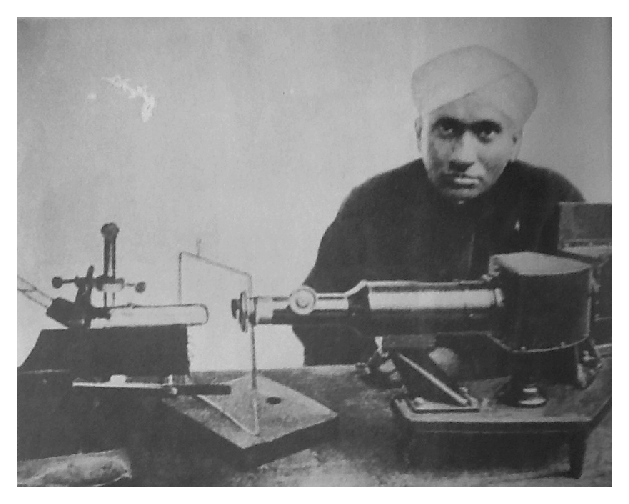
\includegraphics[scale=.9]{eps/1.eps}
\end{center}
\vskip -.5cm
{\fontsize{10pt}{12pt}\selectfont\em Raman with his experimental apparatus used in the discovery of the Raman effect.}\relax

\begin{center}
\includegraphics[scale=.9]{eps/2.eps}
\end{center}
\vskip -.4cm
\centering
{\fontsize{10pt}{12pt}\selectfont\em A modern laser Raman spectrometer.}\relax
\end{figure}

\begin{figure}[H]
\centering
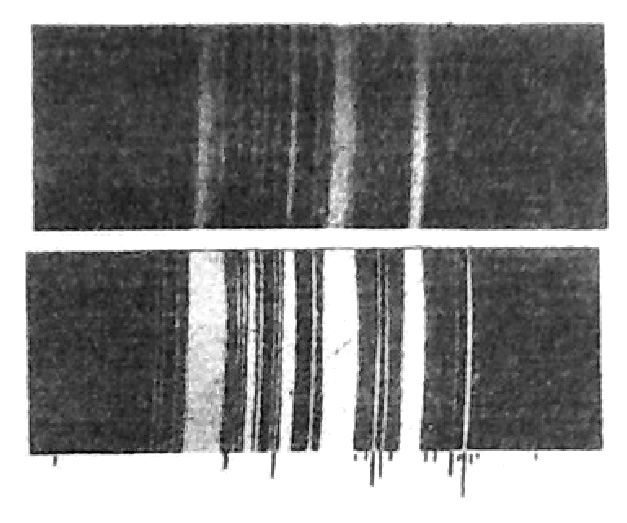
\includegraphics[scale=.77]{eps/2a.eps}
\vskip -.2cm
{\fontsize{10pt}{12pt}\selectfont\em First Raman spectrum, benzene, recorded with mercury arc.}\relax
\vskip -.2cm
\end{figure}


The announcement of the discovery was made to the
Associated Press the following day. Krishnan photographed the
first \hbox{Raman} spectrum with a Hilger Baby Quartz Spectrograph
in which both the Stokes and Antistokes components were
recorded. The note sent to {\em Nature}\index{Nature@\textit{Nature}} on March 8th by Raman and
Krishnan announcing the discovery was rejected by a referee, but
the editor, Sir Richard\break Gregory,\index{Gregory, Richard} published it in the April 21st
issue, accepting the responsibility. Raman gave a full account
of the discovery in public, in an address delivered before the South
Indian Science Association at Bangalore on March 16, 1928. This
address, entitled {\em A New Radiation}, was written immediately on
his return to Calcutta, printed overnight, and one thousand
reprints were posted the same day to scientists all over the world.
Raman and Krishnan quickly realised the nature of the
phenomenon and left out the analogy with the Compton effect\index{Compton Effect}
in subsequent publications. Soon the scientific world got on to the
discovery and the Raman Effect became an active field of research.\index{Raman, Chandrasekhara Venkata!Papers/Publications/Addresses}

Professor Chandrasekhar\index{Chandrasekhar, S.} of the University of Chicago, a
nephew of Raman and at that time a student in the first year
physics honours at Presidency College,\index{Presidency College} Madras, recalls Raman's
visit to their home in Madras on his way to Bangalore to announce
the discovery. ``I remember very well Raman visiting us {\em en route}
to Bangalore, where he was to announce the discovery of his effect
in an address entitled {\em A New Radiation}, before the South Indian
Science Association on March 16, 1928. He was clearly in great
form and he showed us the first spectra of the effect. He was
obviously enthralled that he had discovered the optical analogue
of the Compton effect for which discovery Compton had received
the Nobel Prize in 1927. I remember someone asking him what
could have happened if Raman had discovered his effect a year
earlier. His immediate response was, ``Then I should have shared
the Nobel Prize with Compton and I should not have liked that;
I would rather receive the whole of it''.

Prof. Chandrasekhar spent April, May and June, 1928, in
Calcutta as well as April and May 1929. He records that he
became good friends with many of Raman's associates and
especially with \hbox{Krishnan}. ``The one dominating impression
which was made on me at that time and which has remained with
me is the exhilarating one of being with a group of physicists
in the joy of what everyone recognised as a great discovery,''
he remembers.
\index{Krishnan, K.S.|)}

It is of interest to note here that almost at the same time
as \hbox{Raman} was carrying out his crucial experiments, work on
similar lines was going on in France and Russia. Rocard\index{Rocard} in France
had anticipated, from his theoretical work, a change of wavelength 
in light-scattering due to atomic vibrations of molecule,
and Cabannes\index{Cabannes} and Rocard were looking for the effect in the light
scattered by gases. Gases are poor scatterers and hence they failed
to observe the effect, whereas \hbox{Raman's} work was done with
liquids which turned out to be strong scatterers. When Raman's
first two papers were seen by the French group they immediately
recognized the nature of the phenomenon and quickly realised
its importance to chemical physics.

Quite independently, Landsberg\index{Landsberg} and Mandel'shtam\index{Mandel'shtam} had\break been
working on light-scattering in crystalline quartz and, with\-in a
short time of Raman's announcement of the discovery, these two
Russian physicists came out with their announcement of having
observed a modified line in the scattered spectrum. Raman,
however, had clearly established his priority. From the very
beginning he held the view that scientific results should find
prompt publication and he practiced this throughout his life.
It was precisely for this reason that he created the {\em Indian Journal
of Physics}\index{Indian Journal of Physics@\textit{Indian Journal of Physics}} in Calcutta and started the {\em Proceedings of the Indian Academy of Sciences}\index{Proceedings of the Indian Academy of Sciences@\textit{Proceedings of the Indian Academy of Sciences}} when he shifted to Bangalore.

The apparatus used by Raman for his discovery consisted
of a mirror for deflecting sunlight, a condensing lens, a pair of
complementary glass filters, a flask containing benzene and a
pocket spectroscope, the total cost of which would not have been
more than Rs. 500. It could also be inferred from the account
narrated above that the discovery was not the result of an
accident, but was the culmination of seven years of systematic
and sustained work carried out with devotion by Raman and his
band of students. The achievement is all the more creditable when
it is realised that the support for scientific research in India in
those times was so meagre.

The history of the discovery of the Raman Effect also has
many lessons for the aspirants of Science. It is not very expensive
equipment that is important for making a capital discovery but
the calibre of the scientists, sustained effort and single-mindedness. Hardly any discovery appears right away in its clear
and final form. Nature reveals its secrets bit by bit. Great
discoveries appear incredibly simple only after someone has made
them and explained them.
\index{Raman, Chandrasekhara Venkata!Raman Effect|)}

\medskip
\heading{Sommerfeld's visit to Calcutta}
\addtocontents{toc}{\protect\contentsline{section}{\protect Sommerfeld's visit to Calcutta}{\thepage}}
\vskip .15cm

\index{Sommerfeld, Arnold|(}

\lhead[{\it\fontsize{9pt}{9pt}\selectfont\thepage}]{\it{\fontsize{9pt}{11pt}\selectfont Sommerfeld's visit to Calcutta}}

\noindent
Sommerfeld's visit to India in the latter half of 1928 was
very significant as he was the first physicist of immense stature
to come to Raman's laboratory and see a demonstration of the
new discovery. There were some who expressed doubts as to
whether Raman could have observed such a weak effect.
Sommerfeld came in October 1928 and Raman demonstrated to
him the light-scattering effect he had discovered. Sommerfeld was
tremendously impressed by the experimental demonstration and
the seriousness and dedication with which Raman had been
pursuing his researches.

\vskip .1cm

When Arnold Sommerfeld accepted the invitation to spend
the first few months of 1929 as a guest professor in the United
States of America, he was firmly resolved ``not to take the
ordinary way but the extraordinary one {\em via} the far East''. He
was specially attracted to India, for he had heard about its
wonders, its ancient civilisation and its lofty religious and
philosophical system. Sommerfeld was also impressed with the
strong shoots of modern physics emerging from this part of the
world; he had in mind the emergence of Raman as a world-class
scientist on the verge of discovering the light-scattering effect.
So Sommerfeld planned his detour to India; and this was before
Raman had actually performed the decisive experiment.

\vskip .1cm

\begin{figure}[t]
\begin{center}
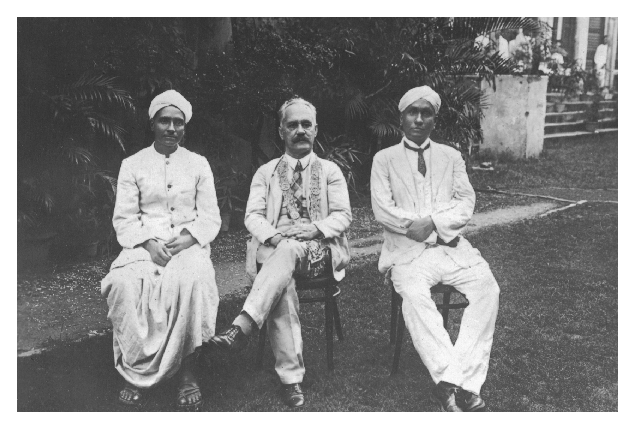
\includegraphics[scale=.95]{eps/3.eps}
\end{center}
\vskip -.4cm
{\fontsize{10pt}{12pt}\selectfont\em Arnold Sommerfeld with C. V. Raman (right) and K.S. Krishnan (left).
Picture taken at Calcutta in 1928. (Photo courtesy of Deutsches Museum, Munich, supplied very kindly by Dr. G. Torkar of Ludwig-Maximilians Universit\"at, Munich.)}\relax
\vskip -.4cm
\end{figure}

Raman had wired Sommerfeld on February 11, 1928:
``Calcutta University inviting you, lecture honorarium thousand
rupees, kindly wire date arrival India.'' When boarding the 
steam-boat in Genoa on August 21, 1928, Sommerfeld carried numerous
invitations, to lecture on Modern Atomic Physics at Indian
universities, as well as an itinerary prepared by Meghnad Saha.\index{Saha, Meghnad}
As soon as he arrived in India he was taken ill and had to be
hospitalised in Bangalore for two weeks. He arrived in Calcutta,
his main destination in India, on October 4, 1928. Several entries
in his diary of the tour speak of his time in Calcutta.
\begin{quote}
{\fontsize{10pt}{12pt}\selectfont
``{\em October 4}: Grand reception at Howrah Station. Raman,
Bose, Krishnan,\index{Krishnan, K.S.} Sen, Gosh., Mitra...also the German vice-consul
Eberl\index{Eberl} at whose place I stay...3 beautiful rooms with
bathroom...hibiscus flowers in blossom up to the first floor...then
Bose takes me to Raman's institute...(he) shows me papers on
diffraction...

{\em October 6}: 8 o'clock in the morning, first special lecture on
Kepler problems, discussion until 10'clock...eventually the Raman
effect visually: blue filter and compl. screen, now put in front
of the incident light, then in front of the scattered light:
difference...

{\em October 7}: Sunday...Wonderful lecture by Raman (also the
rotations of the molecules can be seen unresolved as modified
rad.)...

{\em October 8-13}: Lectures daily from 8-10 with lively
discussions... I saw scattering blue-green on an iceblock in the
institute, obvious modified scattering. Everything in the institute
is very good, but bathroom terrible...
}\relax
\end{quote}

Sommerfeld's interest in India was not restricted to physics.
He was deeply interested in its art as well as the life and the
customs of its people. He left Calcutta on October 14, 1928, to
visit a few other places in Northern India, such as Benares and
Agra. He preferred a trip to Shantiniketan to a sight-seeing tour
through Delhi, following the ``kind'' invitation by the poet and
philosopher Rabindranath Tagore,\index{Tagore, Rabindranath} winner of the Nobel Prize for
Literature. With Tagore, whom he put on a par with Goethe
(Sommerfeld, the humanist, was an ardent admirer of Goethe),
he enjoyed a day of peace, ``the peace of an Indian autumn''.
On October 26th, Sommerfeld left India from Calcutta: ``With
two cars to the harbour. Again a garland of Krishnan and flowers
from the X-ray man...''

During the voyage, he put down the conversation he had
with Raman, on the eve of his departure, and his own
experiences. It is a record in which he comments critically upon
India's economic and political conditions and her difficult
relations with Great Britain. He left India ``in deepest affection
for the highly-gifted, unhappy nation'' and ``with sincere
gratitude for the many acts of friendliness and honourings''. As a
sign of his special gratitude, he proposed Raman as a candidate
for the Nobel Prize. Raman, who learned this, thanked
Sommerfeld effusively: ``I do not know how to express adequately
my gratitude for this act of kindness. The literature of the new
effect is growing at a great pace. I hope the Nobel Committee
may give a favourable decision in December next if my name is
put before them on the occasion also.''

After receiving the Nobel Prize, Raman visited Sommerfeld
in Munich. He was received with great joy: ``We welcome our
guest not only as a successful scientist and discoverer but also
as a representative of the age-old and now rejuvenated culture
of the Orient which trustfully cooperates with the Occidental
culture and strives for the same ends.''

Raman was proposed for the Nobel Prize for Physics in 1929
by N. Bohr\index{Bohr, Niels} and C. Fabry\index{Fabry, C.} and in 1930 by E. Bloch,\index{Bloch, E.} N. Bohr,
L. and M. deBroglie,\index{de Broglie, L. and M.} O. Khvolson,\index{Khvolson, O.} J. Perrin,\index{Perrin, J.} R. Pfeiffer,\index{Pfeiffer, R.}
E. Rutherford,\index{Rutherford, E.} J. Stark\index{Stark, J.} and C.T.R. Wilson.\index{Wilson, C.T.R.} Sommerfeld's
name does not appear in the list of nominators. However, it is
likely that he wrote to the Committee and the recommendation
did not get into the official records. Raman was awarded the Prize
in 1930 and news of the award was hailed universally. Raman,
accompanied by Lady Raman, left for Stockholm, to receive the
Nobel Prize, on December 10, 1930. He was 42 years old.

The meetings of the Nobel Committee are held in the highest
secrecy and the awards announced in November, only about a
month before the prize-giving ceremony in mid-December. Given
the time it would have taken to reach Europe by steam\-ship in
those days, it would have been surprising if Raman could have
reached Stockholm in time for the ceremony if he had arranged
for passage only after receiving the telegram. It is now a historical
fact, however, that \hbox{Raman} had, in anticipation, booked tickets
for himself and his wife\index{Raman, Chandrasekhara Venkata!Raman, Lokasundari} in July that year and it was this that enabled them to reach Stockholm in early December!

\index{Sommerfeld, Arnold|)}

\medskip
\heading{Stockholm and the Nobel ceremony}
\addtocontents{toc}{\protect\contentsline{section}{\protect Stockholm and the Nobel ceremony}{\thepage}}
\smallskip

\lhead[{\it\fontsize{9pt}{9pt}\selectfont\thepage}]{\it{\fontsize{9pt}{11pt}\selectfont Stockholm and the Nobel ceremony}}

\noindent
A vivid eye-witness account of this visit and the Nobel
ceremony in Stockholm was published in the `Raman Number'
of the {\em Calcutta Municipal Gazette}\index{Calcutta Municipal Gazette@\textit{Calcutta Municipal Gazette}} when the Calcutta Corporation
presented an {\em Address to Prof. Raman} in 1931. This fascinating
article, entitled `A week in Stockholm', was written by Lady
Raman\index{Raman, Chandrasekhara Venkata!Raman, Lokasundari} and in it she said:
\begin{quote}
{\fontsize{10pt}{12pt}\selectfont
``The week we stayed in Sweden was one long festival.
If garlanding were as much part of a ceremonial function in
Sweden as in India, the garlands we would have collected would
have been innumerable. But the more common thing there is
photographing. Newspaper reporters were at us even on the boat
taking us to Sweden across the Baltic. I do not know in what
manner the rest of the world looks on the Nobel Laureates, but
the Swedish certainly focus their eyes on them. Parties and
gatherings to meet the Nobel Prizemen are held without
intermission. In India, hospitality is considered to be a religious
duty, but it is in Sweden that I saw what hospitality can be.

Our stay in Stockholm extended for a week from the 9th to
16th\break December, 1930. We arrived by train at Stockholm, the
capital city of Sweden, at 8 o'clock in the morning of the 9th
December. The platform was crowded with people waiting to
receive the guests. There were at least ten cameras ready for
exposure. In northern latitudes in winter, sunlight is a rare
phenomenon, but days and nights are made equally bright by
thousands of electric lights. Everybody who spoke to us expressed
sorrow that it being winter, their country was not looking its best
but was dark and bleak, and that we should see it in spring shining
in sunshine. As their sun never rises high up in the skies, one can
well understand their fondness for sunshine, but if they had
enjoyed the Indian sun of April and May, I am sure their partiality
for the sun would get moderated. Owing to the low actinic value
of electric light they always use flash-light for taking photographs.
The suddenness and attendant noise as of a cracker startle newcomers, 
but we soon got used to it. Not being white-skinned, we
could not mix with the natives of the country without being
recognised; moreover our multi-coloured Indian dress was making
us conspicuous to every eye.

The Scandinavian is of great height and size, and I was
somewhat shy of my comparatively short stature.

Even after reaching the hotel, the stream of photographers
and newspaper reporters continued to show us their attention.
Indians are rare phenomena in Scandinavia and our photographs
were published {\em ad nauseam}. It was very difficult to get rid of the
newspaper men. They must hear about Indian politics; my
husband talked about educational matters, but what was I to talk about? 
I could only speak on the habits, customs and beliefs
of our country. It certainly interested them and they were surprised
about the Hindu ways of living, as I was about their sunless days.''
}\relax
\end{quote}

After referring to the tea at the British Embassy and the
dinner at the Swedish Academy of Sciences,\index{Swedish Academy of Sciences} to which Professor
and Lady Raman\index{Raman, Chandrasekhara Venkata!Raman, Lokasundari} were escorted by Dr. E. Nobel,\index{Nobel, E.} a relative of
Alfred Nobel, Lady Raman described the Nobel Prize Award
Ceremony:
\begin{quote}
{\fontsize{10pt}{12pt}\selectfont
``The\index{Raman, Chandrasekhara Venkata!Awards/Distinctions|(} award of the Nobel Prizes took place on the 10th
December between 4 and 7 p.m. If I shut my eyes, I can still see
as in a dream the great concert hall of Stockholm, decorated with
flowers and flags, filled with more than 4,000 people, the King
and Queen of Sweden and the Royal family occupying the first
seats. The Nobel Laureates then entered the Hall, each
accompanied by a Professor in his own subject and followed by
such Nobel Laureates of previous years as were present in
Stockholm and the members of the Academy. As the procession
entered, the whole audience stood up and remained standing until
the Laureates took their seats amidst a fanfare of trumpets.
The Laureates of the year were seated on one side of the dais and
their introducers on the opposite side. The Secretary of the
Academy of Sciences read a report and gave a brief account of
Nobel's life. Dr. Pleijel,\index{Pleijel, H.} Professor of Electro-Technics in the
University of Stockholm, then rose and spoke for twenty minutes
on my husband's investigations on the scattering of light and the
new effect that had been discovered by him. ({\em Note}: This speech
is given in its entirety at the end of this section.) He then addressed
my husband and said,
\begin{quote}
{\fontsize{10pt}{12pt}\selectfont
`Sir Venkata Raman, The Royal Academy of Sciences
has awar\-ded you the Nobel Prize in Physics for your eminent
researches on the diffusion of gases and for your discovery
of the effect that bears your name. The Raman effect has
opened new routes to our knowledge of the structure of
matter and has already given most important results.'

`I now ask you to receive the prize from the hands of
His Majesty.'}\relax
\end{quote}
On Sir Chandrasekhara rising to receive the Prize, the whole
audience, including the King, stood up and the British flag was
held aloft. The Laureate then approached the Royal Seat and
bowed before the King, who took him by the hand and presented
him the Nobel Medal, Prize and Diploma. This was attended with
loud cheering and was followed by orchestral music for about
fifteen minutes.

Then followed in succession the addresses on the work of
the other Laureates and the award of the medal, prize and diploma
to each of them.

The whole ceremony took about 3 hours and was followed
by the Nobel banquet which took place at the {\em Mela}, a beautiful
building picturesquely situated by the side of the Malar lake. The
banqueting hall can accommodate about 400 guests. The Nobel
Laureates sat at the Royal Table. The dinner was of the most
lavish scale. Wine flowed freely. A few vegetarian dishes had been
considerately provided for us. When it came to the drinking of
health, we had our cups filled with water. In replying to the toast,
Sir Raman spoke of the glories of ancient India. He spoke of the
great renunciation of Buddha, the Royal ascetic and world
teacher, and of his message of non-violence and love which
embraced all living creation. It was nearly twelve when the party
broke up.

Next day, the Nobel lectures were delivered at the University.
Each prize-winner spoke on his own work. These lectures are later
collected in the form of a book. In the evening, there was a
reception by the King and Queen at the Palace. After dinner, the
guests were shown round the library and art collections and time
passed pleasantly in conversation with various members of the
Royal family. We met there a grandson of Tolstoy who kindly
took us to various places of interest.

The 12th December was a very cold day. A chill wind was
blowing. In the night we witnessed an interesting popular festival
called Lucia-light. There was a procession led by a young maid
with a crown of lighted candles on her head. The legend was that
she was heralding the advent of snow and was bringing light for
the dark winter days ahead. Strangely enough, when we woke up
next morning, there was a sheet of white snow all over the city,
greatly enhancing its beauty. Next to Venice, Stockholm is
considered to be the most beautiful city in Europe, with its large
clear fresh-water lake in its centre, magnificent buildings on the
shores of the lake and its clean, broad streets.

As we had few further social engagements, we walked that
morning some distance out of the city to enjoy the beauty of the
snow scenery. The snow had transformed, as if by magic, the dark
artificially lit city and surroundings into a scene of ethereal beauty.

Next day (14th December) we were invited to dinner at the
house of the President of the Swedish Academy, Dr. Petterson.\index{Petterson}
It appears that when the poet Rabindranath Tagore\index{Tagore, Rabindranath} was there,
he sang some Indian songs and the memory of it was still fresh
in their minds. Somehow, they induced my husband to sing!
After one more day of leisured sight-seeing we left for Upsala
on the 16th, where we were the guests of Prof. Siegbahn\index{Seigbahn} and
his lady.''\index{Raman, Chandrasekhara Venkata!Awards/Distinctions|)}
}\relax
\end{quote}

After his return to India from the Nobel ceremony in
Stockholm, Prof. Raman had to face vast crowds of admirers,
anxious to see and hear the great Nobel Prize-winner. He became
such a popular figure in India that, wherever he went, he often
had to address several meetings of citizens and students on his
latest researches and on science in general. This rush of speeches
and public engagements pursued him all through his long life.
{\em The Nobel Presentation Speech by Professor H. Pleijel,\index{Pleijel, H.}
Chairman of the Nobel Committee for Physics of the Royal
Swedish Academy of Sciences}
\begin{quote}
{\fontsize{10pt}{12pt}\selectfont
``Your Majesty, Your Royal Highnesses, Ladies and Gentlemen.

The Academy of Sciences has resolved to award the Nobel
Prize in Physics for 1930 to Sir Venkata Raman for his work on
the scattering of light and for the discovery of the effect named
after him.

The diffusion of light is an optical phenomenon, which has
been\break known for a long time. A ray of light is not perceptible unless
it strikes the eye directly. If, however, a bundle of rays of light
traverses a medium in which extremely fine dust is present, the
ray of light will scatter to the sides and the path of the ray through
the medium will be discernible from the side. We can represent
the course of events in this way; the small particles of dust begin
to oscillate owing to electric influence from the ray of light,
and they form centres from which light is disseminated in all
directions. The wavelength, or the number of oscillations per
second, in the light thus diffused is here the same as in the original
ray of light. But this effect has different degrees of strength for
light with different wavelengths. It is stronger for the short
wavelengths than for the long ones, and consequently it is stronger
for the blue part of the spectrum than for the red part. Hence
if a ray of light containing all the colours of the spectrum passes
through a medium, the yellow and the red rays will pass through
the medium without appreciable scattering, whereas the blue rays
will be scattered to the sides. This effect has received the name
of the\break `Tyndall effect'.

Lord Rayleigh,\index{Rayleigh, Lord} who has made a study of this effect, has put
forward the hypothesis that the blue colours of the sky and the
reddish colouring that is observed at sunrise and sunset is caused
by the diffusion of light owing to the fine dust or the particles
of water in the atmosphere. The blue light from the sky would
thus be light scattered to the sides, while the reddish light would
be light that passes through the lower layers of the atmosphere
and which has become impoverished in blue rays owing to
scattering. Later, in 1899, Rayleigh threw out the suggestion that
the phenomenon in question might be due to the fact that the
molecules of air themselves exercised a scattering effect on the
rays of light.

In 1914 Cabannes\index{Cabannes} succeeded in showing experimentally that
pure and dustless gases also have the capacity of scattering rays
of light.

But a closer examination of scattering in different substances
in solid, liquid, or gaseous form showed that the scattered light
did not in certain respects exactly follow the laws which, according
to calculation, should hold good for the Tyndall effect. The
hypothesis which formed the basis of this effect would seem to
involve, amongst other things, that the rays scattered to the sides
were polarised. This, however, did not prove to be exactly the case.

This divergence from what was to be expected was made the
starting-point of a searching study of the nature of scattered light,
in which study Raman was one of those who took an active part.
Raman sought to find the explanation of the anomalies in
asymmetry observed in the molecules. During these studies of his
in the phenomenon of \hbox{scattering}, Raman made, in 1928, the
unexpected and highly surprising discovery that the scattered light
showed not only the radiation that derived from the primary light
but also a radiation that contained other wavelengths, which were
foreign to the primary light.

In order to study more closely the properties of the new rays,
the primary light that was emitted from a powerful mercury lamp
was filtered in such a way as to yield a primary light of one single
wavelength. The light scattered from that ray in a medium was
watched in a spectrograph, in which every wavelength or
frequency produces a line. Here he found that, in addition to the
mercury line chosen, there was obtained a spectrum of new sharp
lines, which appeared in the spectrograph on either side of the
original line. When another mercury line was employed, the same
extra spectrum showed itself round it. Thus, when the primary
light was moved, the new spectrum followed, in such a way that
the frequency distance between the primary line and the new lines
always remained the same.

Raman investigated the universal character of the
phenomenon by using a large number of substances as a scattering
medium, and everywhere found the same effect.

The explanation of this phenomenon, which has received the
name of the `Raman Effect'\index{Raman, Chandrasekhara Venkata!Raman Effect} after its discoverer, has been found
by Raman himself, with the help of the modern conception of
the nature of light. According to that conception, light cannot
be emitted from or absorbed by material otherwise than in the
form of definite amounts of energy or what are known as `light
quanta'. Thus the energy of light would possess a kind of atomic
character. A quantum of light is proportionate to the frequency
of rays of light, so that in the case of a frequency twice as great,
the quanta of the rays of light will also be twice as great.

In order to illustrate the conditions when an atom emits or
absorbs light energy, we can, according to Bohr,\index{Bohr, Niels} picture to
ourselves the atom as consisting of a nucleus, charged with positive
electricity round which negative electrons rotate in circular paths
at various distances from the centre. The path of every such
electron possesses a certain energy, which is different from
different distances from the central body.

Only certain paths are stable. When the electron moves in
such a path, no energy is emitted. When, on the other hand, an
electron falls from a path with higher energy to one with lower
energy --- that is to say, from an outer path to an inner path ---
light is emitted with a frequency that is characteristic of these two
paths, and the energy of radiation consists of a quantum of light.
Thus the atom can give rise to as many frequencies as the number
of different transitions between the stable paths. There is a line
in the spectrum corresponding to each frequency.

\vskip .1cm

An incoming radiation cannot be absorbed by the atom unless
its light quantum is identical with one of the light quanta that
the atom can emit.

\vskip .1cm

Now the Raman Effect seems to conflict with this law. The
positions of the Raman-lines in the spectrum do not correspond,
in point of fact, with the frequencies of the atom itself, and they
move with the activating ray. Raman has explained this apparent
contradiction and the coming into existence of the lines by the
effect of combination between the quantum of light coming from
without and the quanta of light that are released or bound in the
atom. If the atom, at the same time as it receives from without
a quantum of light, emits a quantum of light of a different
magnitude, and if the difference between these two quanta is
identical with the quantum of light which is bound or released
when an electron passes from one path to another, the quantum
of light coming from without is absorbed. In that case the atom
will emit an extra frequency, which either will be the sum of or
the difference between the activating ray and a frequency in the
atom itself. In this case these new lines group themselves round
the incoming primary frequency on either side of it, and the
distance between the activating frequency and the nearest Raman-lines 
will be identical with the lowest oscillation frequencies of
the atom or with its ultra-red spectrum. What has been said as
to the atom and its oscillations also holds good of the molecule.

\vskip .1cm

In this way we get the ultra-red spectrum moved up to the
spectral line of the activating light. The discovery of the Raman-line
has proved to be of extraordinarily great importance for our
knowledge of the structure of molecules.

\vskip .1cm

So far, indeed, there have been all but insuperable difficulties
in the way of studying these ultra-red oscillations, because that
part of the spectrum lies so far away from the region where the
photographic plate is sensitive. Raman's discovery has now overcome
these difficulties, and the way has been opened for the investigation
of the oscillations of the nucleus of the molecules. We choose the
primary ray within that range of frequency where the photographic
plate is sensitive. The ultra-red spectrum, in the form of the Raman-lines, 
is moved up to that region and, in consequence of that, exact
measurements of its lines can be effected.

In the same way, the ultra-violet spectrum can be investigated
with the help of the Raman Effect. Thus we have obtained a simple
and exact method for the investigation of the entire sphere of
oscillation of the molecules.

Raman himself and his fellow-workers have, during the years
that have elapsed since the discovery was made, investigated the
frequencies in a large number of substances in a solid, liquid and
gaseous state. Investigations have been made as to whether different
conditions of aggregation affect atoms and molecules, and the
molecular conditions in electrolytic dissociation and the ultra-red
absorption spectrum of crystals have been studied.

Thus the Raman Effect has already yielded important results
concerning the chemical constitution of substances; and it is to
foresee that the extremely valuable tool that the Raman Effect
has placed in our hands will in the immediate future bring with
it a deepening of our knowledge of the structure of matter.''}\relax
\end{quote}

\heading{Civic honour by the Calcutta Corporation}
\addtocontents{toc}{\protect\contentsline{section}{\protect Civic honour by the Calcutta Corporation}{\thepage}}
\index{Raman, Chandrasekhara Venkata!Awards/Distinctions|(}
\smallskip

\lhead[{\it\fontsize{9pt}{9pt}\selectfont\thepage}]{\it{\fontsize{9pt}{11pt}\selectfont Civic honour by the Calcutta Corporation}}

\noindent
Among the warm tributes paid to him on his return, that
of the Calcutta Corporation is noteworthy.

\vskip .06cm

The Corporation Address was presented to Sir Chandra\-sekhara
Venkata Raman on Friday, June 26, 1931, at a brilliant function
in the historic Town Hall of Calcutta. The hall was elegantly
decorated and illuminated, and a distinguished gathering, composed
of some of the foremost citizens, was present when the city
fathers, representing the public, acclaimed the Nobel Laureate.

\vskip .06cm

At the head of the staircase, Prof. Raman, accompanied by
Lady Raman, was received by the Aldermen, Councillors and
the principal officers of the Corporation. As he entered the Hall
at the head of the procession, the whole assembly stood up and
greeted him with cheers.

\vskip .06cm

On reaching the dais, the Mayor garlanded, Sir Chandrasekhara, amid applause. As Prof. Raman took his seat, there was
a shower of flowers upon him from an ingenious overhead
contrivance.

\vskip .06cm

To Prof. Raman's right sat the Mayor, while to his left was
seated the Deputy Mayor. Distinguished guests, Aldermen,
Councillors and the principal officers of the Corporation occupied
other seats on the dais. The Mayor then read the Address, which
was printed on {\em Khaddar} with gold embroidery, and presented
it to Sir Chandrasekhara on an engraved silver tray. The Address
was received with applause by the assembly.

\vskip .06cm

Sir Chandrasekhara, who on rising received an ovation,\break made
a striking speech in the course of which he paid a tribute to
Calcutta, which, he said, has been ``the intellectual metropolis
not only of Bengal, or of India, but of the whole of Asia, from
which has gone forth a living stream of knowledge in many
branches of study''.

\vskip .06cm

At the end of the function, the Mayor presented the
Aldermen and Councillors of the Corporation to Sir
Chandrasekhara.

The Corporation offices and schools remained closed on
Thursday, July 2nd, in honour of the presentation of the
Corporation Address to Sir C.V. Raman. This Address read:
\begin{quote}
{\fontsize{10pt}{12pt}\selectfont
``Sir, We, the Aldermen and Councillors of the Corporation
of Calcutta, beg to offer you our respectful congratulations on
your great achievements in the domain of Science. The recent
awards to you of the Nobel Prize, of the Royal Society's Medal
and the Matteucci Medal, are, in each case, the first distinctions
of the kind to be gained by an Asiatic man of Science, and bear
unequivocal testimony to the high esteem and regard in which your
contributions to knowledge are held in the world of Science.
Working in an Indian laboratory, with a purely Indian training,
you have achieved results of the highest value, thus demonstrating
the high level of efficiency attained by this country in the matter
of scientific research.

Your single-minded devotion to the cause of Science and your
bold idealism will ever remain a perennial source of inspiration
to your countrymen. The highest academic degrees and the
lucrative position in Government service, which you won at the
early age of 18, would have satisfied most ambitions. But the
passion for research, which had manifested itself even at that age,
impelled you to seek opportunities for its further expression and
led you to give up a lucrative career for the sake of Science. Your
noble ideal and example have inspired the work of your pupils,
and the {\em Indian Journal of Physics},\index{Indian Journal of Physics@\textit{Indian Journal of Physics}} of which you are the founder,
is the recognised organ for recording and stimulating research in
Physical Science in this country.

It is not for us to narrate the long list of your contributions
to Science, but we may be pardoned for mentioning the Raman
Effect by the discovery of which you have secured a permanent
place in the history of modern Science. New scientific truths,
basing themselves on your epoch-making discovery, are emanating
from the laboratories of every civilised country and continue to
glorify your name.

As a great teacher of the youth of our country, you have
exhibited in a remarkable degree a wide range of intellectual
interests and a gift of exposition often touching the heights of
humour and eloquence.


We recall with pride and pleasure that it was through one
of our eminent fellow citizens that the creative genius of the East
received the homage of the West when the Nobel Prize was
attracted for the first time to Asia by the immortal works of our
great national poet. We rejoice to think that by unravelling the
deep mysteries of Nature, a most distinguished savant of this city
has now brought to the East for the first time the highest award
of the West in the field of Science.

Installed in the Palit Chair of Physics in the University of
Calcutta, you have, by your success in extending the bounds of
human knowledge, supplied some of the most enduring
cornerstones of the City's Temple of Learning. May you, by your
continued efforts, shed further lustre on this City and bring
greater glory to our Motherland, this ancient home of learning
and knowledge.

{\em We beg to subscribe ourselves, Sir, Yours in the service of
the Motherland, The Aldermen and Councillors of the
Corporation of Calcutta: by Bidhan Chandra Roy}

Sir C.V. Raman replied:

``Mr. Mayor, Aldermen and Councillors of the Calcutta
Corporation, Ladies and Gentlemen:-


There are occasions when even the most cold-blooded of men
finds himself deeply moved by emotion. It is possible that the ideal
man of science should be just a perfect thinking machine with
no sentiment or emotion in his make-up. That I am indeed far
from approaching this ideal was evident on a certain occasion in
Stockholm last December when the people of the coldest country
in Europe tendered to a man of science from the tropic East the
highest distinction in their gift. On the present occasion as well,
I have difficulty in finding words in which to convey my feelings.
Permit me, Sir, to express my gratitude to you and your 
Fellow-Councillors for what must be regarded as a supreme honour by
every citizen of Calcutta.

You, Sir, have referred to my early career. It is not often
that the idealism of student days finds adequate opportunity for
expression in the later life of manhood. It will soon be 25 years
from the date of publication of my first research work. That the
scientific aspirations kindled by that early work did not suffer
extinction has been due entirely to the opportunities provided for
me by the great city of Calcutta. To two men, especially, I owe
a debt of gratitude that can never be repaid.

It was the late Dr. Mahendra Lal Sircar,\index{Sircar, Mahendra Lal} who, by founding
the Indian Association for Cultivation of Science,\index{The Indian Association for Cultivation of Science} made it possible
for the scientific aspirations of my early years to continue burning
brightly. Dr. Sircar devoted a life-time of labour to the institution
which he created and equipped in the hope that it would some
day be utilised for the advancement of science in India. Its doors
were open, awaiting the arrival of someone who could utilise the
resources it offered. That arrival happened to be myself.
Dr. Mahendra Lal Sircar did not, alas, live to see his aims
accomplished. He sowed that others might reap.

To another great citizen of Calcutta, a man who was most
farseeing, profoundly gifted and inspired by the highest ideals,
I mean the late Sir Asutosh Mookerjee,\index{Mookerjee, Asutosh} I am also under a deep
debt of gratitude. Sir Asutosh ventured to ask a young and
unknown Government official to throw aside the preferments of
office, and devote himself to the pursuit of knowledge, under the
aegis of the Calcutta University. This, on his part, was an act of
great courage, whereas on mine it was just a case of following
my own inclinations. But for the action which Sir Asutosh took,
my scientific career would long ago have suffered an abrupt
termination.

\newpage

I desire to take this opportunity of expressing my gratitude
also to my many friends in the city of Calcutta who have helped
my work and made my task easier. Amongst them, I wish
particularly to single out my distinguished friend, Sir Prafulla
Chandra Ray, whom I am glad to see here today. I have always
thought it a great privilege to have as my colleague in the Palit
Chair of Chemistry such a distinguished pioneer in scientific
research and education in Bengal as Sir Prafulla Ray.\index{Ray, P.C.} It has been
invariably my experience that I could count on his co-operation
and sympathy in every matter concerning my scientific work.


It has been my good fortune to have had during the past 15
years a long succession of highly gifted collaborators. To them,
also, I am under a deep debt of obligation, for it is their assistance 
that has made possible much of the work that has emerged from
my laboratory. It is generally believed that it is the students who
derive benefit by working under the guidance of a Professor. In
reality, the Professor benefits equally by his association with gifted
students working under him. From the very first, I have acted
under the firm conviction that a Professor who succeeds in
attracting and inspiring a group of co-workers was also benefiting
himself and rendering to the cause of Science far greater service
than he could ever hope to offer in splendid isolation.


You, Sir, have referred to the fact that I never had any
training in foreign laboratories or Universities. I believe myself
that this was a fortunate circumstance, for it is my firm conviction
that the highest inspiration for scientific work is that which comes
from within oneself. It is my earnest hope that it will be possible
in the near future to create opportunities in our own country for
students to do the highest type of creative scientific work. In saying
this, I do not for a moment suggest that we have nothing to learn
from Europe or America, but surely it is better that we learn to
accomplish whatever we can within our own borders.


You, Sir, have said that you desire my association with
Calcutta to be a permanent one. Let me say at once that this is
also my earnest desire. I consider it my great good fortune to have
been a citizen of Calcutta for nearly 25 years. Some have said
that research work cannot be carried on successfully except in cool
climates, such as those of Bangalore or Dehra Dun. A hot day
in June is not an opportune moment to enter upon praise of the
physical climate of Calcutta. But from the point of view of
research, there is something more important than physical climate,
and that is the intellectual climate of the environment. For a
hundred years, Calcutta has been the intellectual metropolis
not only of Bengal, or of India, but of the whole of Asia.
From Calcutta has gone forth a living stream of knowledge in
many branches of study. It is inspiring to think of the long
succession of scholars, both Indian and European, who have lived
in this city, made it their own, and given it of their best. It must
be a profound privilege to be able to work and live in such an
environment.

Of recent years I have had occasions to visit numerous
laboratories abroad. Many of them are being rebuilt or re-organised, 
in order better to cope with the problems of science. 
The Rockefeller Foundation has played the part of a fairy
godmother to many a scientist in Europe and America in the
realisation of his scientific aims and aspirations. It is the Indian
Association for Cultivation of Science\index{The Indian Association for Cultivation of Science} which first afforded me
opportunities for scientific work at Calcutta, and which has been
the scene of the labours of many of my most gifted collaborators.
It is my earnest desire that its laboratory and library should be re-built and re-equipped so as to make their resources comparable
with those of leading institutions abroad. If that desire were
accomplished, not all the appointments in India joined together
and offered to me as one gift would induce me to leave
this great city.

Allow me to thank you once again for the great honour you
have done me.''\index{Raman, Chandrasekhara Venkata!Awards/Distinctions|)}}\relax
\end{quote}

